\section{FSM por comportamiento (estilo \textit{Minimal Bits}) \label{sec:s3}}

\begin{center}
	\begin{minipage}{12cm}
		\begin{tcolorbox}[title=Actividad 3]
			 Describir por comportamiento la FSM del problema que está siendo considerado (como las descripciones vistas en clase). Indicar al compilador usar códigos del registro de estado en forma \textit{``minimal bits''}. Compilar, simular y ver resultado en el visor RTL, ¿se genera el diagrama de estados y la tabla de códigos en los reportes?
			 \enter
			 Para indicar al compilador qué códigos del registro de estado debe usar se debe ir al menú de Quartus correspondiente:\enter
			 
			 $Assignments > Settings > Analysis \& sinthesis > State Machine Processing$
		\end{tcolorbox}	
	\end{minipage}
\end{center}

La visualización RTL de la FSM, descrita por comportamiento en estilo \textit{Minimal Bits}, se muestra en la \autoref{fig:FSM_Behavior_MB_RTL}. En comparación a la Actividad 1 y 2, se implementan solo 2 compuertas lógicas OR, un multiplexor de 4 bits, un selector, un flip-flop D y dos registros de estados. En la \autoref{fig:FSM_Behavior_MB_Graph} se observa el diagrama de estados reportado por el \textit{State Machine Viewer}, que corresponde con el diagrama visto en clase. Además, en la \autoref{fig:FSM_Behavior_MB_Table} se tiene la tabla de códigos utilizada por el software de Quartus, que corresponde al estilo \textit{One-Hot} modificado. Finalmente, en la \autoref{fig:FSM_Behavior_MB_Tran} se hallan todas las transiciones de los estados y que condición se debe dar para hacer el cambio del estado actual al estado destino.

Las simulaciones se visualizan en la \autoref{fig:FSM_Behavior_MB_Wave}. El comportamiento es el mismo que el descrito en actividades anteriores.

En los Anexos se localiza la descripción de la FSM descrita por comportamiento y en estilo \textit{Minimal Bits}. Además de las entradas y salida, se declararon a los 9 estados de la FSM como parámetros, así como dos registros, uno para almacenar el estado actual y otro para el siguiente estado. En una lista sensible se detectan a los flancos de subida de CLK y de bajada de RST y dentro de esta, empleando una estructura \textit{case}, se describió el comportamiento de cada estado y el estado destino de acuerdo al valor de la señal entrada W.

\begin{figure}[ht]
	\centering
	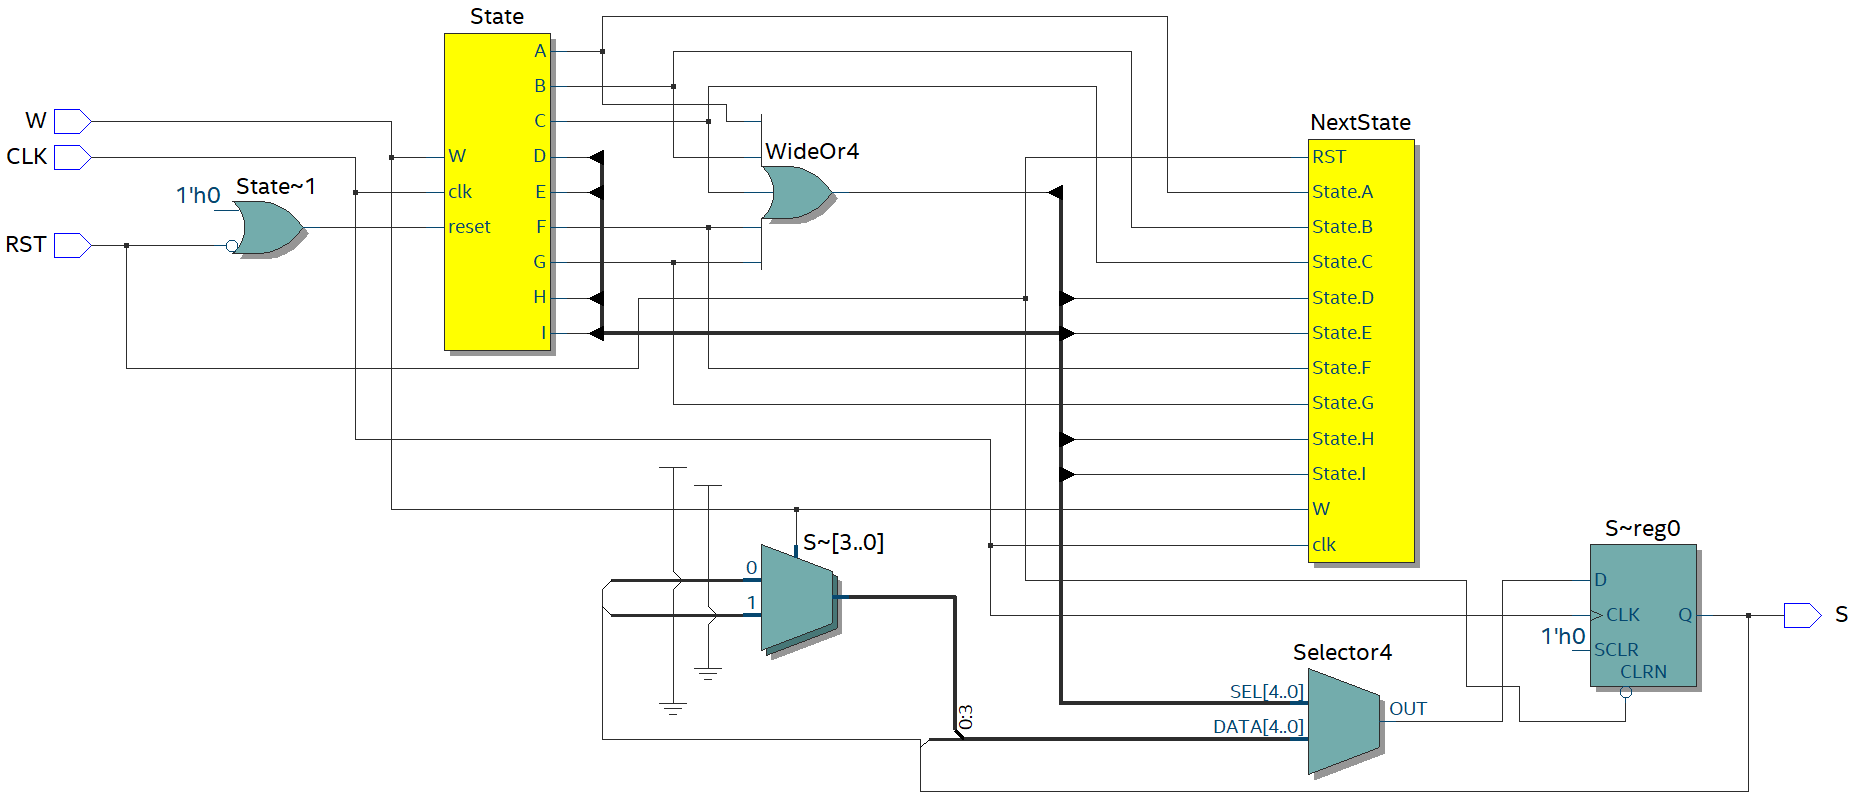
\includegraphics[scale=0.34]{FSM_Behavior_OneHot_RTL.png}
	\caption{Diagrama RTL de la FSM, descrita por comportamiento en codificación \textit{Minimal Bits}. \label{fig:FSM_Behavior_MB_RTL}}
\end{figure}

\begin{figure}[ht]
	\centering
	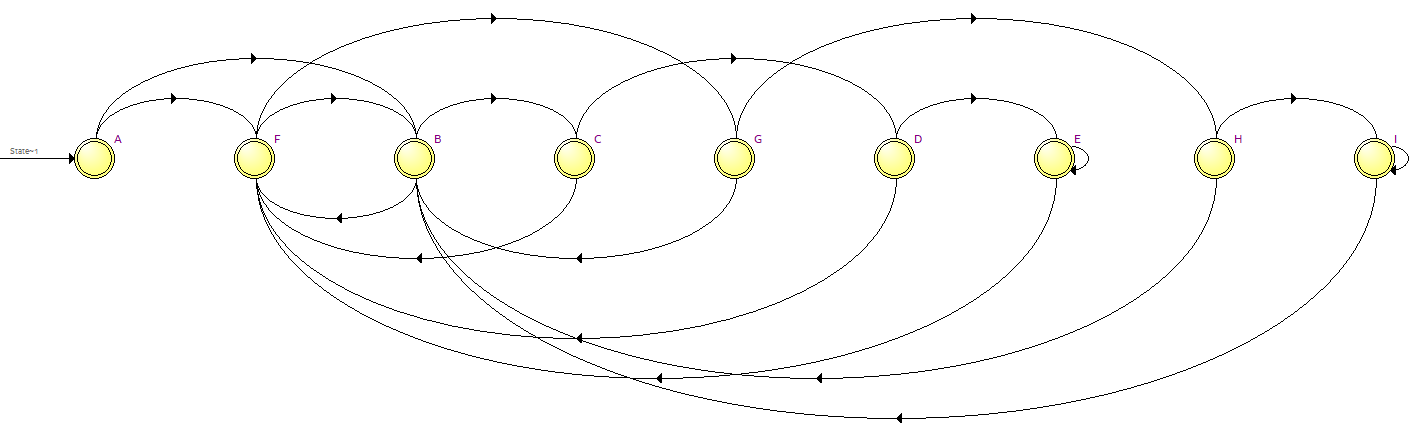
\includegraphics[scale=0.45]{FSM_Behavior_OneHot_Graph.png}
	\caption{Diagrama de estados generado por el \textit{State Machine Viewer} de la FSM estilo \textit{Minimal Bits}. \label{fig:FSM_Behavior_MB_Graph}}
\end{figure}

\begin{figure}[ht]
	\centering
	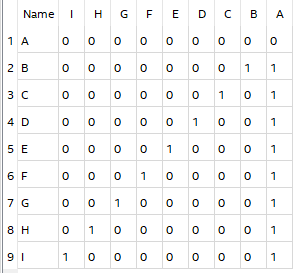
\includegraphics[scale=0.8]{FSM_Behavior_OneHot_Table.png}
	\caption{Tabla de códigos (tipo \textit{One-Hot} modificado) generada por el \textit{State Machine Viewer} de la FSM estilo \textit{Minimal Bits}. \label{fig:FSM_Behavior_MB_Table}}
\end{figure}

\begin{figure}[ht]
	\centering
	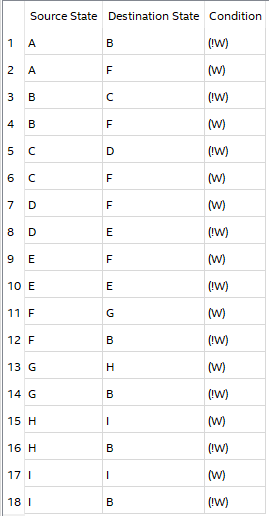
\includegraphics[scale=1.2]{FSM_Behavior_OneHot_Tran.png}
	\caption{Tabla de transiciones generada por el \textit{State Machine Viewer} de la FSM estilo \textit{Minimal Bits}. \label{fig:FSM_Behavior_MB_Tran}}
\end{figure}

\begin{figure}[ht]
	\centering
	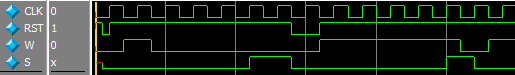
\includegraphics[scale=1.2]{FSM_OneHot_Wave.png}
	\caption{Simulación de la FSM estilo \textit{Minimal Bits}, en el visor de formas de onda de ModelSim. \label{fig:FSM_Behavior_MB_Wave}}
\end{figure}